%!TEX root = main.tex

\section{Experiments and numerical results}

\subsection{Experimental setup}
\begin{figure}[h!]
  \centering
    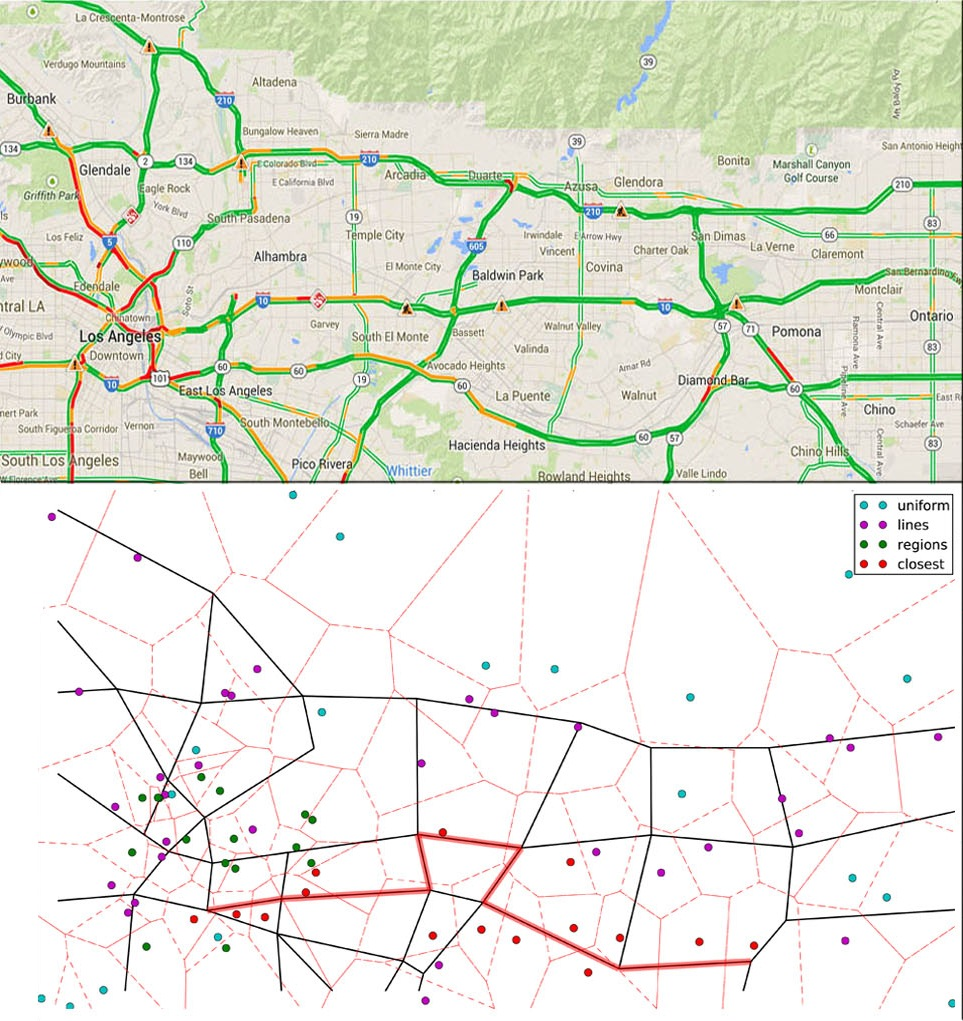
\includegraphics[width=0.47\textwidth]{figures/small_map_half.jpeg}
  \caption{\footnotesize{Benchmark example network based off of the Highway network of the I-210 highway corridor in L.A. county (top, from Google Maps); Network with 80 sampled cells, with a higher concentration of cells near downtown (bottom). A random path from is shown in red with the closest cell towers.}}
  \label{fig:small-network}
\end{figure}

We consider a medium sized network based off of the I-210 highway corridor in Los Angeles, CA (see Figure \ref{fig:small-network}) in the following scenarios, where $N$ indicates the number of uniformly sampled cellular tower positions. 
\begin{itemize}
\item \textit{Urban sprawl} ($N=300$): We emulate a city network where the density of cell towers is sufficient for recovering route flow in the noiseless setting.
\item \textit{City Center} ($N=375$): We emulate a popular commercial district with a very dense sampling.
\end{itemize}
In each of the scenarios, we first compute a feasible route flow $x$ for the user equilibrium solution of the network. Treating $x$ as our sampling distribution, we issue 10,000 vehicles and collect the cellpath flow following the noise model described in Section \ref{sec:system-model}. We fix the parameters $\alpha\in\set{0,0.05,0.1}, \beta=\set{0, 0.05, 0.1, 0.2, 0.3},\xi=\set{0, .0004, .0008, .0012, .002}$. For each configuration, we use the projected first-order method solver in \cite{Wu2015} to compute $x_{est}$. We evaluate on the metric $\norm{x-x_{est}}_1/\norm{x}_1$, which corresponds to the percent route flow error.

\subsection{Preliminary results}

We present preliminary numerical results in Figure \ref{fig:results1}.

\begin{figure}[h!]
  \centering
    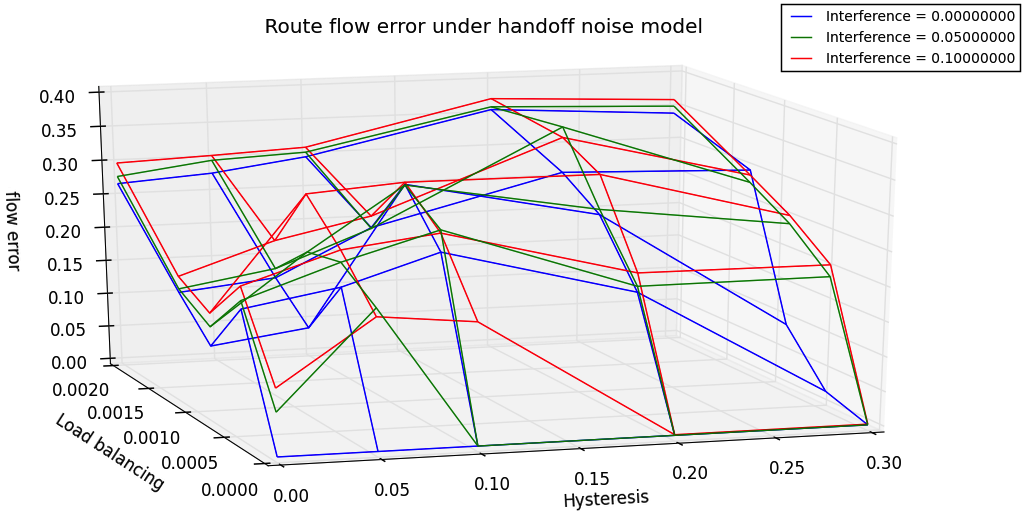
\includegraphics[width=0.47\textwidth]{figures/results_300_hysteresis.png}
  \caption{\footnotesize{This plot show the initial findings for $N=300$. In general, the percent route flow error increases as the interference increases. The percent route flow error first increase then decreases as the hysteresis margin is increased. The load balancing parameter indicates positive correlation with percent route flow error.}}
  \label{fig:results1}
\end{figure}

“sparser”: smallest number of cell towers for which route flow accuracy is pretty good ($<5\%$ error); hopefully somewhat robust to handoff model

“city center”: super dense number of cell towers; handoff model should cause tons of problems here quickly

